%%%%%%%%%%%%%%%%%%%%%%%%%%%%%%%%%%%%%%%%%%%%%%%%%%%%%%%%%%%%%%%%%%%%%%%%%%%%%%
%%%%%%%%%%%%%%%%%%%%%%%%%%%%%%%%%%%%%%%%%%%%%%%%%%%%%%%%%%%%%%%%%%%%%%%%%%%%%%
%%
%%%%%%%%%%%%%%%%%%%%%%%%%%%%%%%%%%%%%%%%%%%%%%%%%%%%%%%%%%%%%%%%%%%%%%%%%%%%%%
%%%%%%%%%%%%%%%%%%%%%%%%%%%%%%%%%%%%%%%%%%%%%%%%%%%%%%%%%%%%%%%%%%%%%%%%%%%%%%
\documentclass[12pt,a4paper,titlepage,final]{article}
\newcommand{\uv}[1]{\quotedblbase #1\textquotedblleft}
% cestina a fonty
\usepackage[czech]{babel}
\usepackage[utf8]{inputenc}
% balicky pro odkazy
\usepackage[bookmarksopen,colorlinks,plainpages=false,urlcolor=blue,unicode]{hyperref}
\usepackage{url}
% obrazky
\usepackage[dvipdf]{graphicx}
\usepackage{listings} 
% velikost stranky
\usepackage{graphicx}
\usepackage[top=3.5cm, left=2.5cm, text={17cm, 24cm}, ignorefoot]{geometry}

\begin{document}

\begin{titlepage}

\begin{figure}[h]
\begin{center}

\includegraphics[scale=0.6]{logo.eps}
\end{center}
\end{figure}

\begin{center}
\LARGE
\textsc{Vysoké učení
  technické v~Brně\\ \Large{Fakulta informačních technológií}}\\
\vspace{\stretch{0.382}}
\LARGE
SHO Štátna volebná infraštruktúra \\
\Huge
Dokumentácia z predmetu IMS\\ 
\large{\medskip
\today }\\
\vspace{\stretch{0.618}}
\end{center}
 \hfill   

\begin{flushleft}
\begin{large}
\begin{tabular}{ll}
\textbf{Autori:} \\ \\

Martin Maga  xmagam00, \\Vojtěch Meca   xmecav00 \\ \\


\end{tabular}
\end{large}
\end{flushleft}
\end{titlepage}


\tableofcontents
\newpage

\section{Úvod}
Táto dokumentácia sa zaoberá vývojom, implementáciou a testovaním systéum hromadnej obsluhy "Štátna volebná infraštruktúra", ktorá simuluje volebný systém v Českej republike zahrňujúci voľby v okrskov a krajských mestskách a následne odoslanie a počítanie hlasov v informačnom centre.
\indent
Na základe modelu a simulácie bude ukázané chovanie systému so zreteľom na ukázanie slabých miest pri voľbách. Tento projekt môže byť použitý na optimalizáciu systému voliev v Českej republike vzhľadom na zrychlénie celého systému počítania hlasov a rozdelenie do okrskov.

\subsection{Autori}
Na projekte SHO "Štátna volebná infraštruktúra" sa podieľali nasledujúci autori:
\begin{itemize}
\item Martin Maga(xmagam00)
\item Vojtěch Meca(xmecav00)
\end{itemize}

Okrem vyššie spomenutých ľudí sme využili možňosť konzultácie s pánom doktorom Hrubým(konzultácia ohľadne správnosti nášho návrhu Petriho siete).

\subsection{Testovacie prostredie}
Pre testovacie účely boli použité architekrúry:Linux 3.2.0-56-generic $86_64$ GNU/Linux pre menšie vzorky dát a pre rozsiahlejšie testovanie na väčšej vzorke dát: FreeBSD eva.fit.vutbr.cz 9.2-STABLE FreeBSD amd64.

\subsection{Validita}
Experimentovaním sme overovali validitu modelu, ktoré vo forme histogramu a jeho následnej analýze odpovedali nášhu odhadovanému predpokladu. Tak isto sme využili dostupné informácie o spôsoboe volieb v Českej republiky a štatistických informáciách, ktoré sú verejne prístupné na internete.

\subsection{Zadanie}
Obsah zadania: "Státní volební infrastruktura nechť se skládá z volebního informačního centra a sítě volebních okrsků. Centrum přijímá zprávy od volebních okrsků a prezentuje výsledky v jednotlivých krajích (nutno modelovat server centra jako obslužnou linku). Volební okrsky jsou SHO obsahující obslužné linky: komise a místo pro provedení volby do obálky ("za plentou"). Modelujte proces příchodů voličů v průběhu doby voleb. Volební komise skončí práci buď po odvolení všech občanů v okrsku nebo okamžikem konce volebního víkendu. Potom sčítá hlasy (doba je závislá na počtu obálek v urně) a odesílá výsledky do centra. Prostudujte systém voleb v ČR a síť volebních okrsků. Konkrétní síť okrsků generujte náhodně s následujícím omezením: sumární počet voličů v krajích musí odpovídat realitě a počet voličů v krajských městech musí odpovídat realitě. Okrsky nějak vhodně agregujte tak, aby jejich celkový počet byl cca 200. Náhodně generovanou síť okrsků uložte do souboru a experimenty provádějte stále nad stejným modelem sítě okrsků. Zdokumentujte model sítě okrsků. Na experimentech ukažte propustnost centra, doby čekání okrsků na připojení do centra, celkovou dobu práce lidí okrskových komisích."
Obsah je dostupný online z nasledujúceho odkazu: http://perchta.fit.vutbr.cz:8000/vyuka-ims/31.\cite{Prokop:Algoritmy}



\subsection{Ciele projektu}
Ciele projektu zahŕňajú:
\begin{itemize}
\item Analýza aktuálneho volebného systému v Českej republike
\item Analýza slabých miest volebného systému
\item Návrh efektívnejšieho prístupu, ktoré by dokázalo zvýšiť rýchlosť počítania hlasov
\end{itemize}


\section{Rozber témy a použitých technológií}

\indent


Pre zobrazenie výsledkov bola použitá trieda Histogram, ktorá je štandardnou súčasťou knižnice Simlib.


\subsection{Popis použitých postupov}
Pre implementáciu bol zvolený jazyk C++ a knižnicu určenú na simuláciu Simlib. Toto rozhodnutie bolo učinené na základe formálnych požiadavok na tvorbu projektu. Ďalším kritériom bola aj široká ponuka prostriedkov, ktoré knižnica Simlib ponúka na simuláciu modelov. Ďalej treba spomenúť, že kód v C++ je pomerne rýchly.



\subsection{Pôvod použitých technológií}
\begin{itemize}
\item Simlib -http://www.fit.vutbr.cz/~peringer/SIMLIB/ (GNU LGPL)
\item C++ - http://en.wikipedia.org/wiki/C++
\item Ubuntu - http://www.ubuntu.com/
\item Petriho siete - $http://en.wikipedia.org/wiki/Petri_net$
\item GNU PLOT - $http://www.gnuplot.info/$

\end{itemize}
\subsection{Volebný systém v Českej republike}
Česká republika sa zaraďuje medzi dvojkomorové parlamentné 
systémy. Tvorí ju Poslanecká snemovňa a Senát. Do PS ČR sa volí na 
základe pomerného voličského systému. Základnú reguláciu nájdeme 
v Ústave ČR. V čl. 18 nachádzame základné princípy volieb, ako je spôsob 
voľby tajným hlasovaním na základe všeobecného, rovného a priameho 
práva, podľa zásad pomerného zastúpenia. Ďalším dôleţitým zákonom je 
zákon č. 247/1995 Sb., o voľbách. Niektoré ustanovenia sú prevedené 
vyhláškou č. 233/2000 Sb. Tieto právne pramene sú základnými právnymi 
prameňmi v oblasti volieb v ČR.\cite{Seda:Voleb}

Voľby prebiehajú štandardne každé 4 roky, alebo po po predčasných voľbách. Každému občanovi republiky prislúcha 1 volebný hlas, ktorý musí odovzdať. Každý občas patrí pod istý volebný kraj, ktorý sa delí na menšiu časti zvané okrsky. Voľby prebiehajú štandardne v sobotu alebo v nedeľu dokopy 14 hodín. Každý občan, ktorý spĺňa podmienky príde v mieste svojho bydliska do volebnej miestnosti, kde sa preukáže platnosti dokladom totožnosti volebnej komisii, ktorá skontroluje údaje a povolí občanovi voliť. Každý občan ide jednotlivo za urnu, kde zaškrtne možnosť a následne vhodí svoj hlas do urny a zvyšné zahadzuje.

Na konci volieb sú hlasí v jednotlivých okrskoch sčítané a odnesené na obecný úrad, odkiaľ sa posielalu na prepočítanie do lebného centra.

  







\section{Koncepce - modelářska témata}
Na obrázku č. ... je uvedeno schéma systému Volební infrastruktury.\newpage 
\begin{figure}[h]

\begin{center}

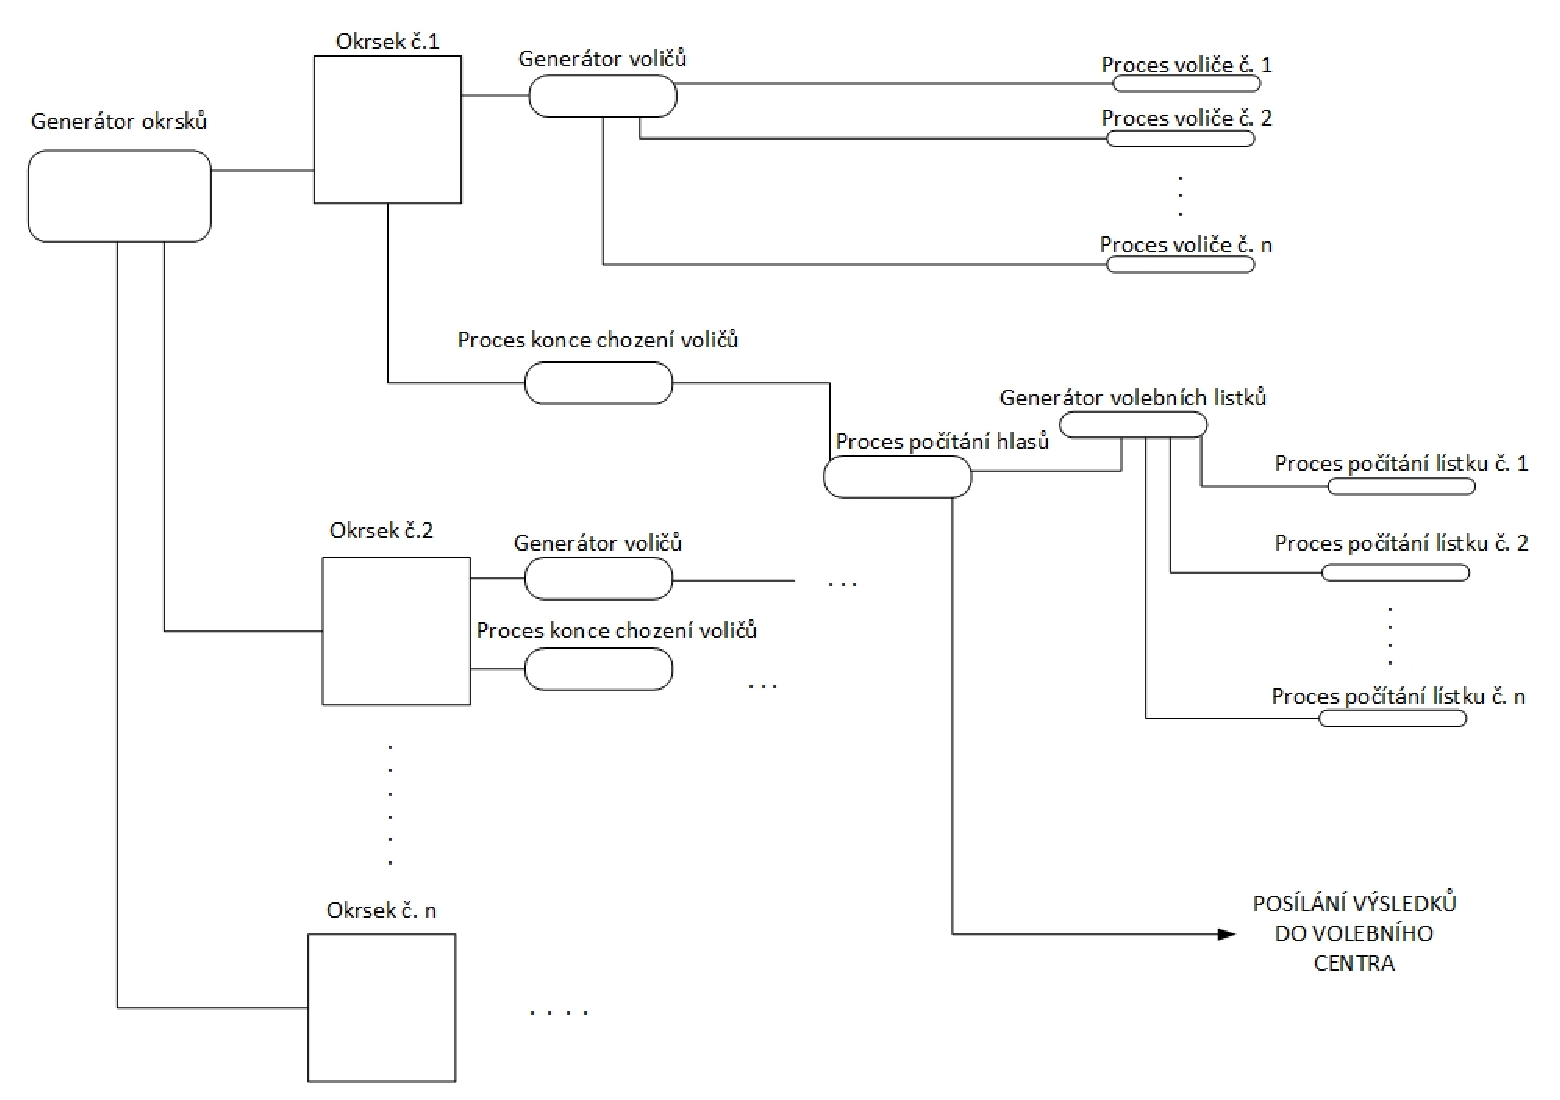
\includegraphics[scale=0.7]{img/konceptualni_model.eps} 
\caption{Konceptuálny model}
\label{koncept}

\end{center}

\end{figure}

\newpage

\subsection{Opis konceptuálneho modelu}
 

\newpage 
\begin{figure}[h]

\begin{center}

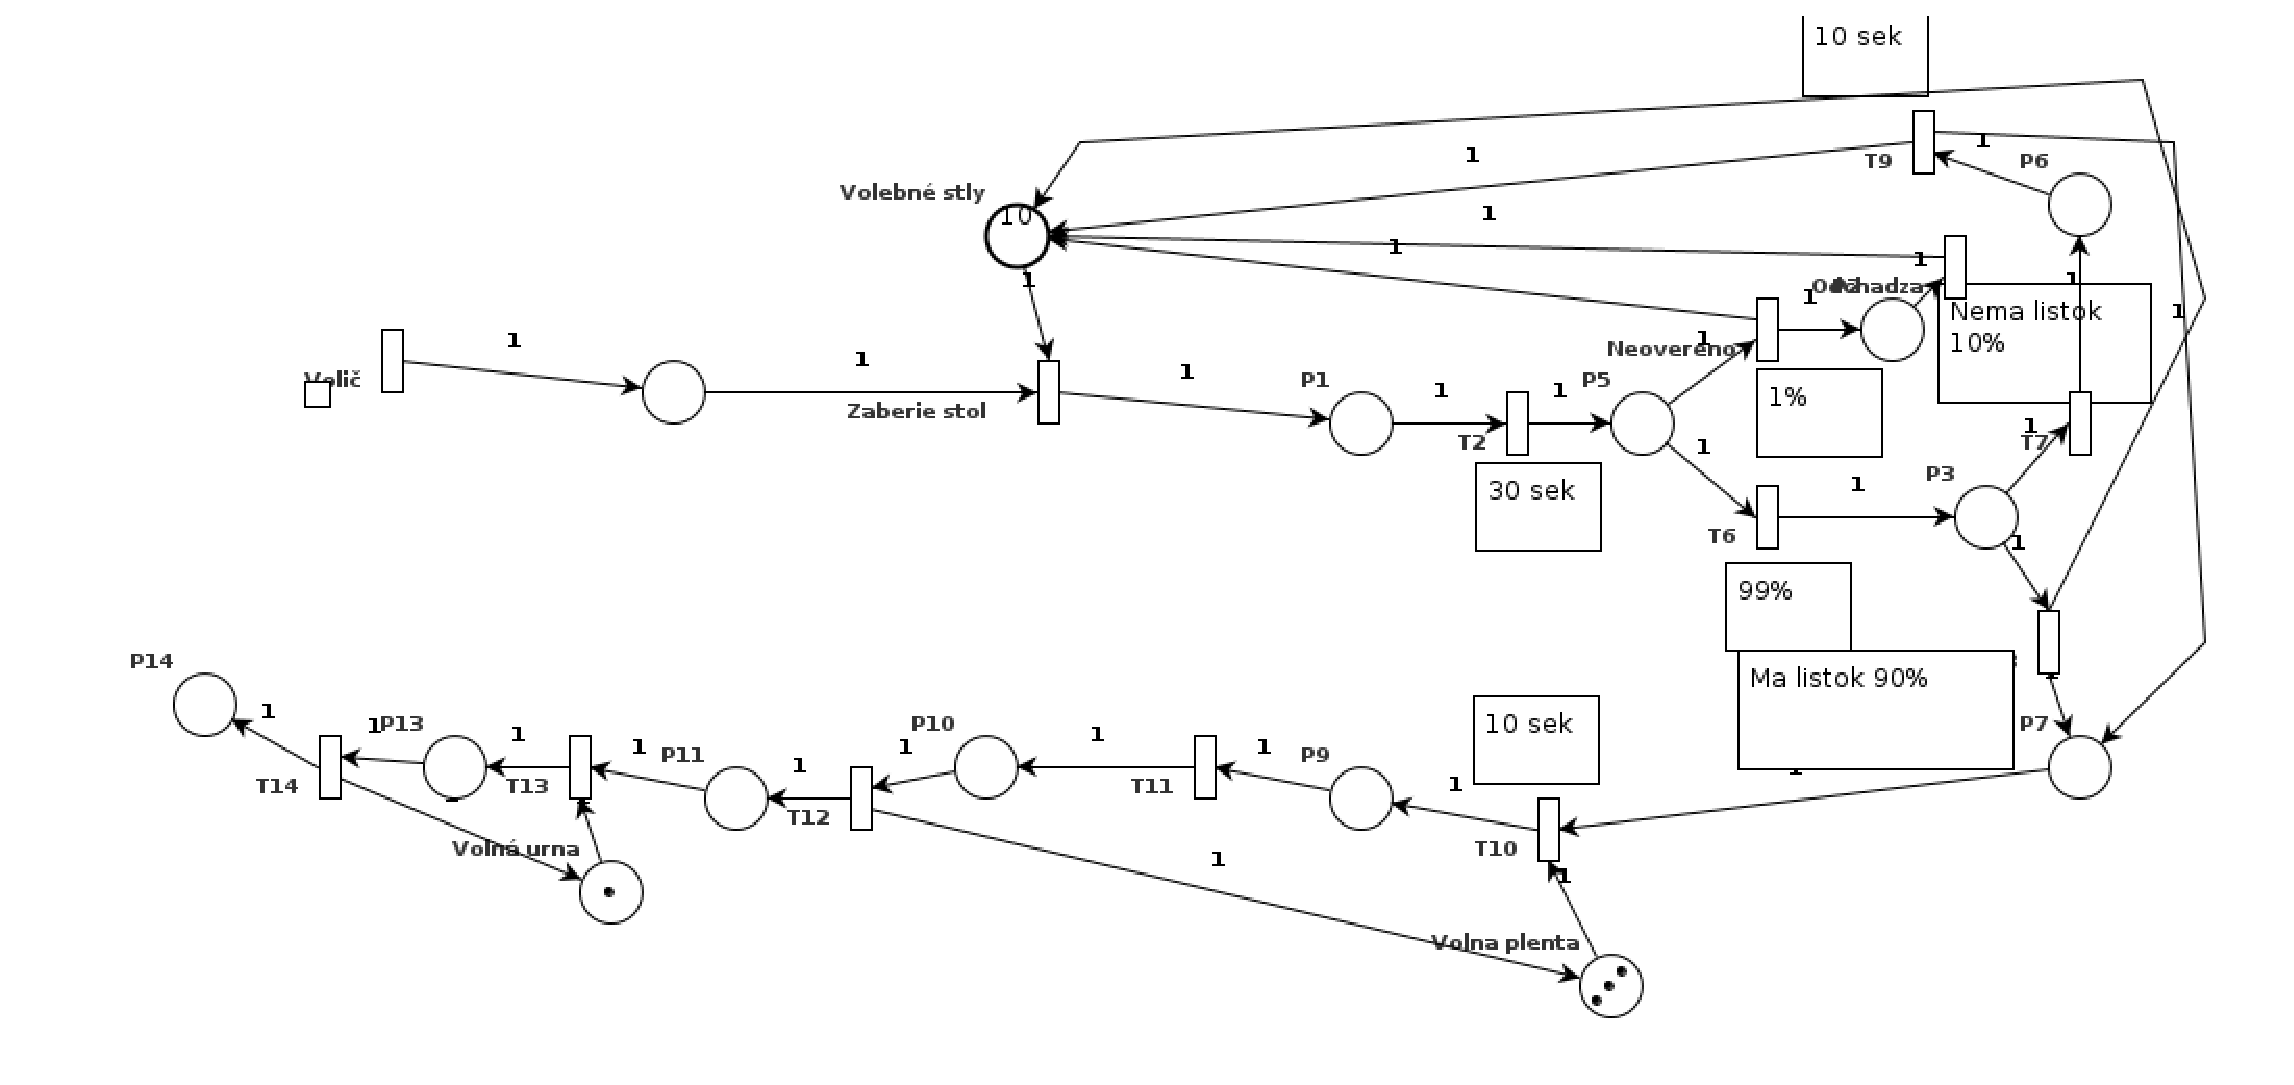
\includegraphics[scale=0.4]{img/Petri.eps} 
\caption{Konceptuálny model}
\label{koncept}

\end{center}

\end{figure}

Obrázok popisuje Petriho sieť, ktorá ukazujem systém volieb. Ukazuje príchod voliča, odvolenie voliča. Na začiatku sa vygenerujú voliči, ktorí prijdu do volebnej miestnosti. Pri vstupe do miestnosti si občan zabere člena volebnej komisie, ktorý je reprezentovaný štruktúrou "Store" s kaúacitou 10 v Simlibe. Pokiaľ nie je voľný nejaký člen volebnej komisie, tak si občan zabere frontu podľa minimálnej dĺžky. Pokiaľ sa občan dostane na rad, tak ho člen volebnej komisie skontroluje. To trvá 20 sekúnd. V prípade, že občan má občiansky tak môže pokračovať vo voľbách. V opačnom prípade(1\,\%) užívateľ odchádza. Inak občan pokračuje ďalej. Zabere si "Store" s kapacitou 3, ktorí reprezentuje volebnú plentu. V prípade, že nie je volná plenta, tak sa občan zaradí do najkratšej fronty. Následne užívateľ zajde za plentu a zaškrtá výsledok. To trvá cca 10 sekúnd. Následne si zabere plentu, ktorá je len 1. Pokiaľ nie je voľná tak sa zaradí do fronty a čaká. Následne občan opúšťa systém.
\newpage


\subsection{Forma konceptuálneho modelu}


\subsection{Implementácia}
Program pracuje na základním procesu, který regeneruje v čase nula objekty reprezentující okrsky České republiky. Při vytvoření objektu jednotlivého okrsku se nainicializují data. Objekt reprezentující okresek po inicializaci spustí po sobě jdoucí 2 procesy. První z nich je proces, který po svém vzniku začne generovat procesy příchodů voličů do volební místnosti. Druhý z procesů vytvoří časovač, který udává legální délku voleb. Po uplynutí určeného času na příchod voličů tento proces vytvoří nový proces. Nově vytvořený proces se stará o počítání jednotlivých volebních lístků ve volební místnosti, dále simuluje kontrolu výsledků a taky posílání správně vypočtených výsledků do Volebního centra České Republiky. Problém počítání jednotlivých volebních lístků řeší pomocí procesu na generování procesu počítání volebního lístku. V případě, že po spočítání výsledků se zjistí, že nastala chyba v počtech, proces zopakuje počítání volebních lístků znovu. 




\section{Architektura simulačního modelu}
\newpage


\section{Podstata simulačných experimentov}

\section{Zhrnutie simulačných experimentov a záver}

\subsection{Testovanie}
Testovanie nášho projektu prebiehalo na architektúrach Windows a Linux. Bolo založené na vopred napísaných testoch, ktoré porovnávali jednotlivé výsledky testovanej časti s~referenčnými. Testovanie spočiatku prebiehalo po častiach, tak ako boli postupne implementované jednotlivé časti intepretu.
V~konečnej fáze boli vykonané komplexné testy, ktoré overili funkčnost nášho interpretu jazyka \emph{IFJ12} podľa špecifikácie uvedenej v~zadaní. V~prípade, že bola objavená chyba počas testovania, táto chyba bola ihneď odstránená a interpret bol opäť dôkladne otestovaný.


\subsection{Štatistiky}
\newpage


 
\newpage




\newpage

\section{Referencie}


\bibliographystyle{czechiso}

\bibliography{dokumentace}
\newpage
\end{document}

